\begin{figure}
  \centering
  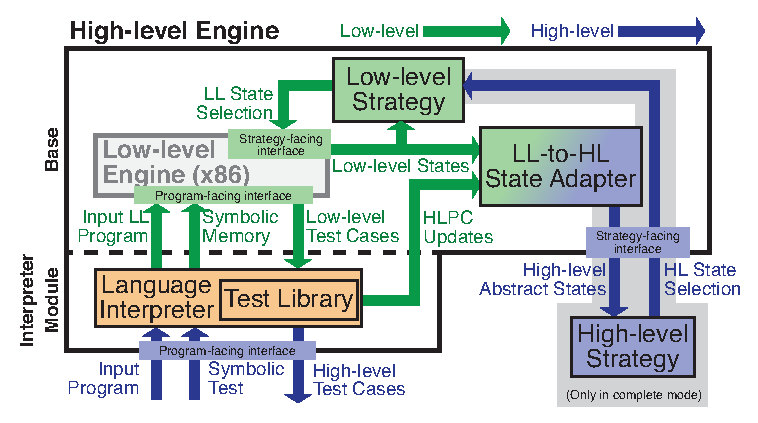
\includegraphics[width=0.8\textwidth]{chef/figures/iface-adapter}
  \caption{The architecture of \chef.}
  \label{fig:chef:arch}
\end{figure}

\chef acts as an adapter between two symbolic execution engine interfaces:
%
the user-facing \emph{high-level} engine interface that receives the target program and the internal \emph{low-level} binary engine that runs the interpreter.
%% %
%% The main function of \chef is to prioritize the low-level interpreter states that maximize the effectiveness of test case generation at the high-level.

The interface of a symbolic execution engine consists of a program-facing part and a strategy-facing part.
%
Through the program-facing part, the symbolic execution engine receives the program and the symbolic test and outputs test cases.
%
Through the strategy-facing part, the engine sends the active execution states to an external state selection strategy and receives the choice of the next state to run (see Section~\ref{sec:intro:symbex}).


Figure~\ref{fig:chef:arch} shows the architecture of \chef, consisting of the base and an interpreter module.
%
The base contains the \emph{low-level} binary symbolic execution engine (S2E) that runs the interpreter, its state selection strategy, and an \emph{adapter} that converts from the low-level interpreter paths to the high-level program paths.
%
An external high-level strategy communicates with the base to provide the next high-level state to run.

The interpreter module contains the language interpreter, which provides the implicit semantics of the language.

Both the inner and the outer interfaces of \chef expose the program-facing and the strategy-facing part.
%
The inner engine operates with machine-level abstractions: it runs a binary program---the interpreter---and marks memory bytes as symbolic inputs.  During symbolic execution, it generates paths through the interpreter binary, prioritized by the low-level strategy.
%
The outer engine operates with corresponding high-level abstractions: it runs an interpreted program and marks objects, instead of bytes, as symbolic.  During execution, it generates paths through the high-level program.

The interpreter module \emph{by construction} adapts the program-facing part of the two interfaces, as shown in Figure~\ref{fig:chef:arch}.
%
Reusing the interpreter provides substantial savings in terms of development effort.  For instance, the Python interpreter has over 400 KLOC; an equivalent hand-written symbolic execution engine would reimplement from scratch the same language semantics in an implementation of the same order of magnitude.

The main task left for \chef is to provide the low-level strategy for choosing the interpreter paths that maximize \chef's effectiveness as a high-level symbolic execution engine.
%
We discuss this aspect in the next section.

%%% Local Variables: 
%%% mode: latex
%%% eval: (visual-line-mode)
%%% fill-column: 1000000
%%% TeX-master: "main"
%%% End:
